\documentclass{article}
\usepackage{amssymb}
\usepackage{babel}
\usepackage{geometry}
\usepackage{amsmath}
\usepackage{amsthm}
\usepackage{framed}
\usepackage{pifont}
\usepackage{listings}
\usepackage{graphicx}
\usepackage{subcaption} 
\usepackage{subcaption} 


\def\ra{\rightarrow}
\def\oo{\infty}
\def\l/{\backslash}
\def\0{\emptyset}
\def\b{\,\,\,}
\def\mm{{\mu^*}}
\def\hm{\mathcal{H}^s}
\def\vm{\nu^*}
\def\cui{\bigcup_{i=1}^\infty}
\def\cai{\bigcap_{i=1}^\infty}
\def\cuj{\bigcup_{j=1}^\infty}
\def\caj{\bigcap_{j=1}^\infty}
\def\sumj{\sum_{j=1}^\infty}
\def\sumi{\sum_{i=1}^\infty}
\def\sumn{\sum_{n=1}^\infty}
\def\px{\mathcal{P}_X}
\def\s{\mathcal{S}}
\def\a{\mathcal{A}}
\def\bs{\mathcal{B}}
\def\lm{\mathcal{L}}
\def\R{\mathbb{R}}
\def\E{\mathbb{E}}
\def\Z{\mathbb{Z}}
\def\m{\mathcal{M}}
\def\rr{\Rightarrow}
\def\tf{$\Rightarrow$}
\def\f{\mathcal{F}}
\def\limn{\lim_{n \rightarrow \infty}}
\def\st{\text{s.t.}}
\def\sums{ \sum_{x \in \s}}

%Ricky Def
\def\baru{\bar{\mu}}
\def\Mbaru{\mathfrak{M}_{\baru}}


\title{COMP4211 PA1 Report} 
\author{Name: Ruiming Min; SID: 20827430; ITSC: rmin}
\date{\today}

\begin{document}

    
\maketitle

\section*{Part 1: Data Exploration and Preparation}

\subsection*{Q1.}
\begin{itemize}
    \item The training set contains 3539 samples(instances), each with 31 features and 2 labels.
    \item The 1-st to 6-th, 8-th to 14-th and 16-th features are categorical, while the rest are numerical.
\end{itemize}

\subsection*{Q2.}

\subsubsection*{The missing values and the percentage of missing values for each feature:}
% draw a dable to show the missing values and the percentage of missing values
\begin{center}
    \begin{tabular}{|c|c|c|}
        \hline
        Feature & Missing Values & Percentage of Missing Values \\
        \hline
        1 & 29 & 0.819441\% \\
        5 & 49 & 1.384572\% \\
        6 & 108 & 3.051710\% \\
        9 & 82 & 2.317039\% \\
        10 & 142 & 4.012433\% \\
        12 & 158 & 4.464538\% \\
        13 & 170 & 4.803617\% \\
        14 & 120 & 3.390788\% \\
        16 & 138 & 3.899407\% \\
        18 & 148 & 4.181972\% \\
        21 & 171 & 4.831873\% \\
        23 & 16 & 0.452105\% \\
        24 & 28 & 0.791184\% \\
        26 & 144 & 4.068946\% \\
        30 & 160 & 4.521051\% \\
        \hline
    \end{tabular}
    \newline
    \textbf{P.S.: If the feature is not listed in the table, then it has no missing values.}
\end{center}

\subsubsection*{The effect of missing values on the distribution of the features:}
Since the missing values may make the information less compheresive, which may lead more bias. These missing values may make the distribution of the features biased, and may also affect the performance of the model. 

\subsection*{Q3.}
\subsubsection*{Numerical:}
The 15-th, 17-th 19-th, 20-th, 22-rd, 25-th and 27-th features are discrete. The rest are continuous. 
\begin{center}
    \begin{tabular}{|c|c|c|c|c|}
        \hline
        Feature & Mean & Standard Deviation & Median & Range\\
        \hline
        First N-Feature (7-th)  & 66.324696  & 6.619953 & 66.55& 47.5~95 \\
        Second N-Feature (15-th)  & 23.204012 & 7.427675 & 20 & 17~70 \\
        Third N-Feature (17-th)  & 0.683526 & 2.275012 & 0 & 0~20 \\
        \hline
    \end{tabular}
\end{center}

Boxplot for the three numerical features:
% import the pic from ./pic/boxplot.png
\begin{figure}[h]
    \centering
    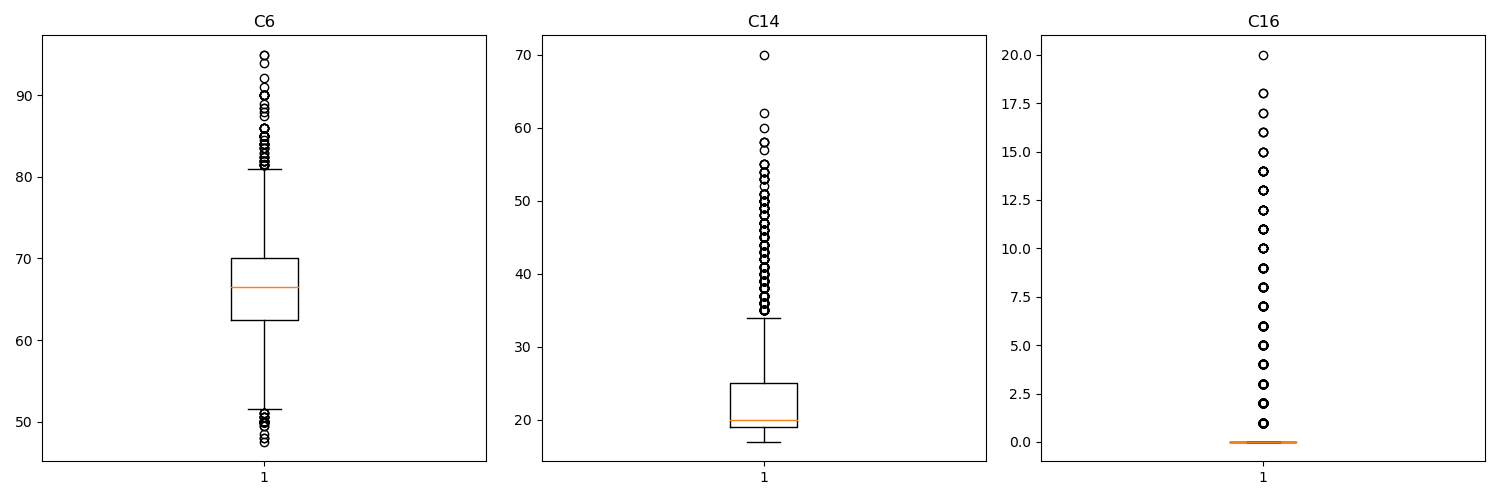
\includegraphics[width=0.8\textwidth]{./pic/boxplot.png}
    \caption{Boxplot for the three numerical features}
\end{figure}

\subsubsection*{Categorical:}
Binary features indexes (from 1): 5, 9, 10, 11, 12, 13, 14, 16.\\
Nominal features indexes (from 1): 1, 2, 4, 8.\\ 
Ordinal features indexes (from 1): 3, 6.\\



\begin{table}[h!]
    \centering % 确保表格整体居中
    \begin{subtable}[t]{0.4\textwidth}
        \centering % 子表格内容居中
        \begin{tabular}{|c|c|}
            \hline
            Value & Count \\
            \hline
            single    & 3115 \\
            married  & 296 \\
            divorced & 75 \\
            facto union & 18 \\
            legally separated & 3 \\
            widower & 3\\
            \hline
        \end{tabular}
        \caption{\textbf{1st Categorical Feature:}} % 子表格标题
    \end{subtable}
    %\hfill % 使用 \hfill 来确保子表格之间有空间
    \begin{subtable}[t]{0.4\textwidth}
        \centering % 子表格内容居中
        \begin{tabular}{|c|c|}
            \hline
            Value & Count \\
            \hline
            second choice   & 2402 \\
            third choice & 457 \\
            fourth choice  & 247 \\
            fifth choice & 194 \\
            sixth choice & 125 \\
            seventh choice & 112 \\
            last choice  & 1 \\
            first choice  & 1 \\
            \hline
        \end{tabular}
        \caption{\textbf{3rd Categorical Feature:}} % 子表格标题
    \end{subtable}

\end{table}

\begin{table}[h!]
        \centering % 子表格内容居中
        \small
    \begin{tabular}{|c|c|}
        \hline
        Value & Count \\
        \hline
        1st phase - general contingent   & 1351 \\
        2nd phase - general contingent & 708 \\
        Over 23 years old  & 630 \\
        Change of course & 253 \\
        Technological specialization diploma holders & 160 \\
        Holders of other higher courses & 109 \\
        3rd phase - general contingent  & 105 \\
        Transfer & 67 \\
        Change of institution/course & 45 \\
        Short cycle diploma holders  & 30 \\
        1st phase - special contingent (Madeira Island) & 29 \\
        International student (bachelor) & 26 \\
        1st phase - special contingent (Azores Island) & 14 \\
        Ordinance No. 854-B/99 & 7 \\
        Ordinance No. 612/93 & 2 \\
        Ordinance No. 533-A/99, item b3 (Other Institution) & 1 \\
        Ordinance No. 533-A/99, item b2) (Different Plan) & 1 \\
        Change of institution/course (International) & 1 \\
        \hline
        
    \end{tabular}
    \caption{\textbf{2nd Categorical Feature:}}  
\end{table}

% import the pic from ./pic/categorical.png
\begin{figure}[h!]
    \centering
    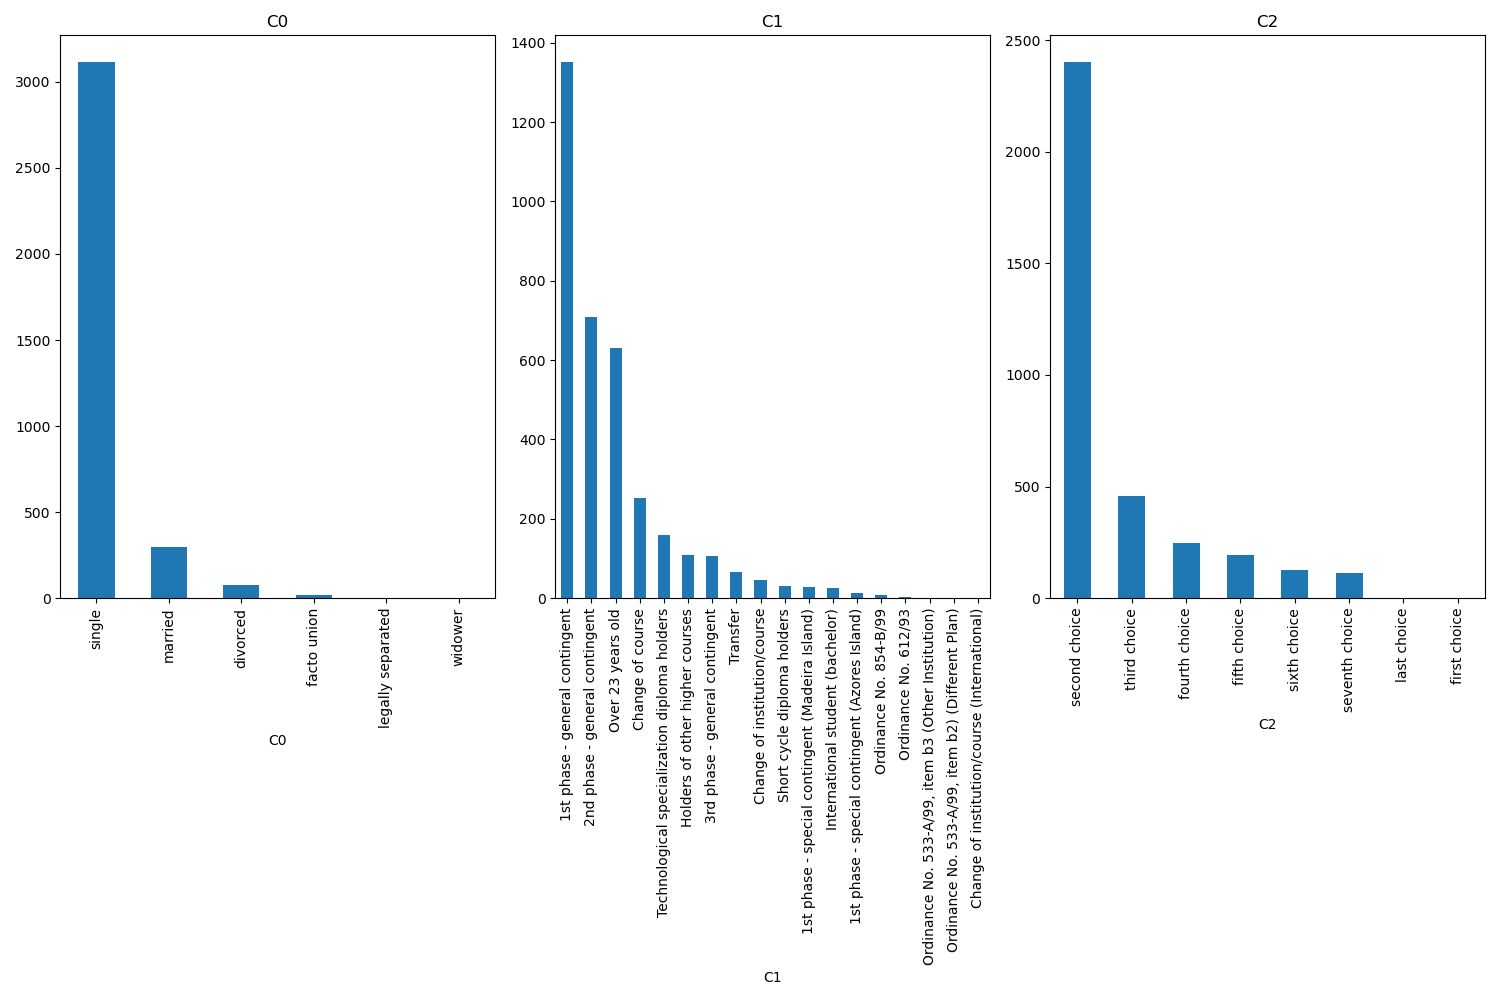
\includegraphics[width=0.8\textwidth]{./pic/categorical.png}
    \caption{Barplot for the three categorical features}
\end{figure}

\newpage

\subsection*{Q4.}
\subsubsection*{Detection:}
Z-Score:\\
\begin{itemize}
    \item Outliers Index of First N-Feature (7-th): 59,  176,  207,  342,  971, 1156, 1840, 2272, 2282, 2447, 2448, 2535, 2624, 3259, 3300, 3373, 3487, 3490
    \item Outliers Index of Second N-Feature (15-th): 99,  252,  278,  280,  291,  394,  403,  432,  513,  553,  607, 
    687,  695,  719,  722,  790,  985,  987, 1018, 1036, 1214, 1233,
    1244, 1266, 1316, 1388, 1408, 1455, 1508, 1512, 1515, 1573, 1581,
    1647, 1691, 1725, 1756, 1782, 1891, 1892, 1906, 1966, 1972, 2020,
    2119, 2125, 2126, 2140, 2178, 2195, 2260, 2317, 2406, 2450, 2509,
    2557, 2613, 2650, 2674, 2702, 2731, 2787, 2827, 2831, 2856, 2895,
    2930, 3048, 3069, 3075, 3077, 3111, 3112, 3126, 3187, 3210, 3327,
    3343, 3412
    \item Outliers Index of Third N-Feature (17-th):18,   33,   83,  150,  152,  173,  278,  337,  362,  391,  424,
    474,  493,  508,  513,  516,  522,  526,  549,  552,  555,  586,
    609,  643,  657,  683,  771,  783,  851,  909,  912,  916,  947,
   1106, 1112, 1174, 1180, 1189, 1240, 1243, 1244, 1298, 1299, 1316,
   1364, 1412, 1428, 1429, 1440, 1463, 1507, 1524, 1541, 1576, 1581,
   1589, 1602, 1632, 1647, 1699, 1789, 1797, 1843, 1847, 1855, 1876,
   1884, 1931, 1965, 1986, 2015, 2054, 2075, 2100, 2122, 2224, 2242,
   2279, 2335, 2339, 2377, 2430, 2455, 2459, 2535, 2555, 2625, 2674,
   2676, 2684, 2698, 2716, 2757, 2764, 2804, 2814, 2821, 2827, 2913,
   2920, 2950, 3045, 3050, 3053, 3064, 3068, 3086, 3273, 3354, 3376,
   3448, 3470, 3500, 3528
\end{itemize}

IQR:\\

\begin{itemize}
    \item Outliers Index of First N-Feature (7-th): 18, 20, 59, 77, 93, 101, 114, 171, 176, 201, 207, 278, 307, 322, 323, 330, 342, 382, 387, 472, 498, 508, 523, 537, 542, 549, 553, 583, 607, 635, 721, 745, 764, 776, 786, 795, 796, 803, 807, 821, 848, 912, 971, 987, 1021, 1031, 1036, 1054, 1156, 1182, 1194, 1217, 1224, 1235, 1244, 1261, 1284, 1307, 1333, 1386, 1390, 1407, 1451, 1482, 1485, 1516, 1571, 1602, 1628, 1629, 1669, 1683, 1711, 1747, 1840, 1851, 1861, 1871, 1884, 1890, 1892, 1932, 1944, 1966, 1972, 1985, 2026, 2047, 2050, 2051, 2177, 2178, 2197, 2256, 2263, 2272, 2282, 2293, 2333, 2373, 2391, 2411, 2413, 2415, 2422, 2447, 2448, 2535, 2539, 2598, 2616, 2622, 2624, 2675, 2737, 2756, 2763, 2773, 2803, 2809, 2816, 2835, 2915, 2968, 3003, 3043, 3072, 3085, 3144, 3153, 3194, 3206, 3236, 3259, 3260, 3272, 3278, 3300, 3317, 3332, 3370, 3373, 3427, 3431, 3487, 3490, 3536.
    \item Outliers Index of Second N-Feature (15-th): 0, 3, 40, 47, 49, 85, 99, 117, 133, 136, 160, 173, 215, 236, 244, 252, 255, 278, 280, 291, 305, 307, 309, 311, 332, 362, 374, 390, 391, 394, 403, 416, 419, 430, 432, 465, 468, 474, 480, 492, 500, 507, 513, 515, 516, 521, 523, 525, 526, 545, 552, 553, 560, 564, 598, 600, 605, 607, 633, 635, 638, 644, 653, 668, 675, 687, 695, 719, 722, 726, 729, 730, 737, 739, 754, 764, 768, 771, 790, 806, 828, 848, 851, 864, 881, 985, 987, 1018, 1029, 1032, 1036, 1051, 1105, 1114, 1124, 1140, 1147, 1156, 1182, 1214, 1217, 1233, 1239, 1244, 1246, 1248, 1254, 1264, 1266, 1287, 1305, 1316, 1351, 1368, 1370, 1377, 1380, 1381, 1388, 1398, 1406, 1408, 1421, 1453, 1455, 1462, 1479, 1481, 1504, 1508, 1512, 1515, 1525, 1569, 1573, 1581, 1586, 1591, 1592, 1602, 1623, 1637, 1644, 1647, 1648, 1654, 1663, 1671, 1673, 1678, 1691, 1704, 1717, 1725, 1732, 1745, 1749, 1754, 1755, 1756, 1765, 1782, 1784, 1789, 1791, 1795, 1799, 1824, 1836, 1855, 1861, 1867, 1886, 1891, 1892, 1906, 1924, 1931, 1949, 1966, 1969, 1971, 1972, 1974, 1985, 1996, 1997, 2020, 2042, 2047, 2053, 2094, 2101, 2106, 2117, 2119, 2122, 2125, 2126, 2130, 2140, 2144, 2171, 2177, 2178, 2189, 2195, 2197, 2198, 2225, 2226, 2230, 2243, 2260, 2270, 2284, 2290, 2316, 2317, 2332, 2369, 2373, 2377, 2386, 2398, 2406, 2410, 2411, 2420, 2442, 2449, 2450, 2459, 2466, 2481, 2491, 2502, 2509, 2529, 2535, 2557, 2559, 2567, 2571, 2574, 2591, 2595, 2611, 2613, 2634, 2650, 2663, 2669, 2674, 2686, 2702, 2714, 2731, 2751, 2758, 2764, 2773, 2787, 2803, 2827, 2829, 2831, 2842, 2851, 2853, 2856, 2857, 2858, 2864, 2865, 2885, 2895, 2906, 2909, 2930, 2943, 2952, 2963, 2965, 2995, 2997, 3003, 3023, 3037, 3048, 3069, 3070, 3072, 3075, 3076, 3077, 3084, 3092, 3095, 3102, 3106, 3111, 3112, 3118, 3126, 3144, 3148, 3159, 3163, 3172, 3187, 3207, 3210, 3224, 3236, 3264, 3284, 3289, 3309, 3323, 3327, 3335, 3343, 3376, 3380, 3382, 3388, 3393, 3397, 3399, 3412, 3415, 3431, 3434, 3448, 3463, 3484, 3499, 3518, 3523
    \item Outliers Index of Third N-Feature (17-th): 5, 12, 14, 17, 18, 27, 33, 44, 48, 53, 58, 66, 74, 83, 86, 92, 101, 121, 126, 144, 150, 152, 156, 160, 164, 166, 169, 173, 174, 200, 210, 223, 243, 246, 253, 267, 278, 288, 298, 304, 317, 322, 324, 327, 335, 336, 337, 353, 358, 362, 391, 404, 409, 412, 424, 429, 430, 438, 444, 456, 472, 474, 479, 493, 495, 508, 509, 513, 516, 522, 526, 534, 549, 552, 555, 561, 564, 586, 598, 605, 609, 612, 614, 618, 635, 637, 643, 649, 654, 657, 660, 662, 675, 683, 687, 721, 726, 739, 744, 754, 762, 765, 766, 770, 771, 781, 783, 798, 801, 811, 812, 814, 834, 843, 847, 851, 860, 870, 909, 911, 912, 914, 916, 946, 947, 958, 970, 985, 987, 989, 992, 1001, 1020, 1021, 1030, 1044, 1051, 1073, 1091, 1095, 1101, 1106, 1112, 1113, 1122, 1139, 1145, 1156, 1160, 1174, 1179, 1180, 1183, 1189, 1197, 1233, 1240, 1243, 1244, 1253, 1277, 1289, 1298, 1299, 1304, 1305, 1311, 1313, 1316, 1323, 1361, 1362, 1364, 1366, 1381, 1395, 1404, 1412, 1419, 1428, 1429, 1440, 1458, 1463, 1464, 1467, 1472, 1490, 1494, 1497, 1504, 1505, 1507, 1509, 1524, 1537, 1541, 1568, 1573, 1576, 1581, 1589, 1591, 1595, 1602, 1603, 1623, 1632, 1638, 1644, 1645, 1647, 1652, 1655, 1659, 1668, 1699, 1708, 1714, 1720, 1722, 1735, 1748, 1766, 1772, 1776, 1784, 1785, 1789, 1791, 1794, 1797, 1805, 1806, 1808, 1812, 1814, 1815, 1821, 1822, 1827, 1841, 1843, 1847, 1855, 1858, 1861, 1863, 1867, 1876, 1884, 1894, 1897, 1898, 1904, 1921, 1922, 1926, 1931, 1950, 1965, 1966, 1974, 1986, 1987, 2002, 2004, 2005, 2012, 2013, 2015, 2016, 2031, 2039, 2054, 2055, 2075, 2080, 2086, 2100, 2106, 2109, 2122, 2160, 2171, 2172, 2173, 2189, 2211, 2214, 2224, 2225, 2235, 2236, 2242, 2244, 2248, 2260, 2267, 2279, 2303, 2319, 2326, 2329, 2330, 2333, 2334, 2335, 2339, 2341, 2351, 2356, 2361, 2376, 2377, 2383, 2386, 2395, 2398, 2411, 2422, 2430, 2432, 2434, 2436, 2455, 2459, 2471, 2480, 2481, 2494, 2499, 2504, 2511, 2519, 2534, 2535, 2555, 2571, 2576, 2581, 2586, 2598, 2604, 2625, 2635, 2644, 2650, 2665, 2674, 2676, 2684, 2686, 2689, 2692, 2698, 2716, 2729, 2735, 2742, 2743, 2756, 2757, 2764, 2773, 2782, 2787, 2793, 2801, 2804, 2806, 2814, 2816, 2821, 2823, 2827, 2832, 2856, 2860, 2866, 2876, 2891, 2906, 2913, 2920, 2930, 2947, 2950, 2994, 2996, 3009, 3020, 3024, 3032, 3045, 3050, 3053, 3054, 3060, 3064, 3065, 3068, 3085, 3086, 3104, 3137, 3156, 3160, 3171, 3179, 3209, 3215, 3249, 3251, 3273, 3278, 3283, 3284, 3285, 3286, 3295, 3300, 3301, 3303, 3307, 3309, 3315, 3325, 3335, 3346, 3354, 3360, 3375, 3376, 3388, 3393, 3399, 3405, 3416, 3432, 3436, 3437, 3444, 3448, 3468, 3470, 3484, 3485, 3493, 3499, 3500, 3512, 3528, 3534
\end{itemize}

\subsubsection*{Consideration:}
Since too many outliers may influence the mean and standard deviation, and the distribution of the data. The outliers may also affect the performance of the model.

\subsection*{Q5.}
\subsubsection*{Feature correlation:}

The following is the heatmap (Figure \ref{fig:heatmap}) for the correlation matrix of the numerical features:
% import the pic from ./pic/heatmap.png
\begin{figure}[h!]
    \centering
    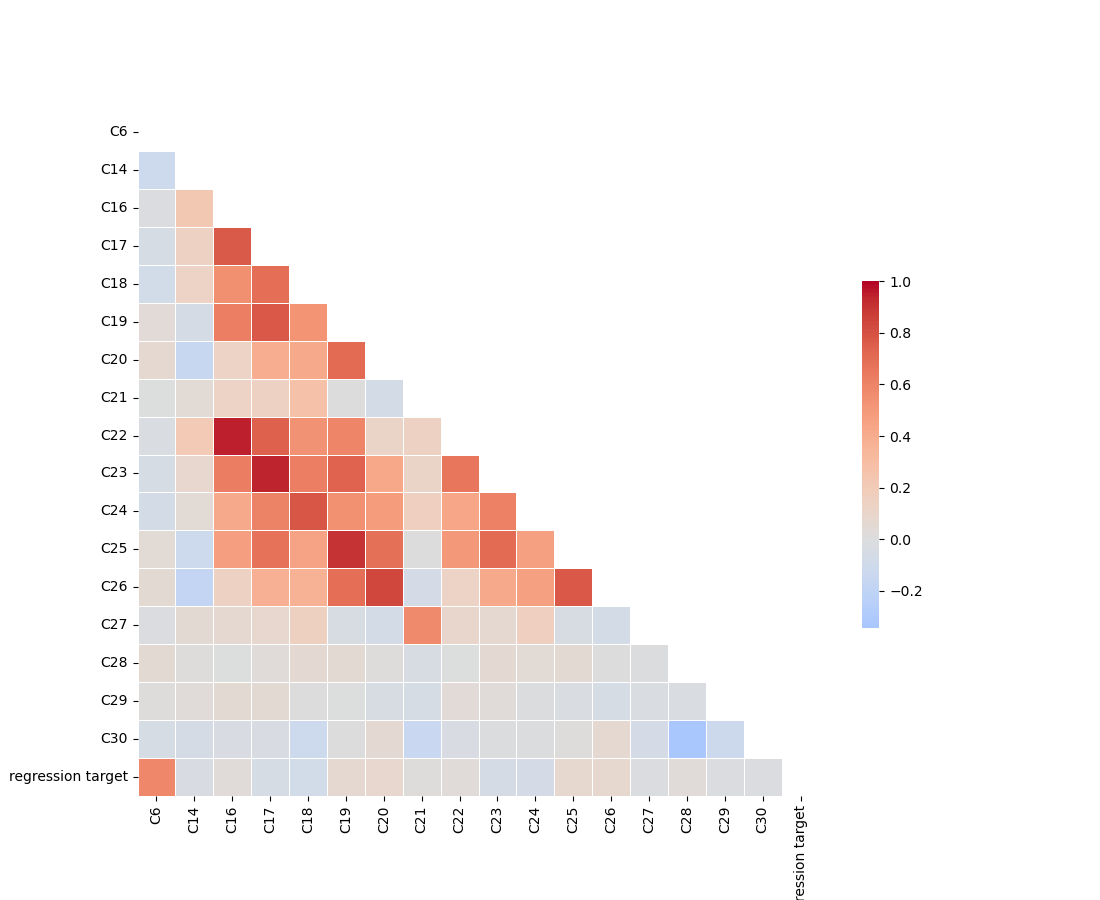
\includegraphics[width=0.8\textwidth]{./pic/heatmap.png}
    \caption{Heatmap for the correlation matrix}
    \label{fig:heatmap}
\end{figure}


\subsubsection*{Insights:}
The following pairs of features are highly correlated (correlation coefficient $> 0.7$):\\
Features C16 and C17 have a correlation of 0.76\\
Features C20 and C26 have a correlation of 0.84\\
Features C16 and C22 have a correlation of 0.94\\
Features C23 and C25 have a correlation of 0.70\\
Features C19 and C20 have a correlation of 0.71\\
Features C19 and C25 have a correlation of 0.90\\
Features C17 and C22 have a correlation of 0.75\\
Features C25 and C26 have a correlation of 0.77\\
Features C17 and C23 have a correlation of 0.94\\
Features C17 and C19 have a correlation of 0.77\\
Features C19 and C23 have a correlation of 0.73\\
Features C18 and C24 have a correlation of 0.78\\

Since these features are highly correlated, we may consider to remove some of them to avoid the multicollinearity.
We can also use PCA, UMAP or tSEN to reduce the dimensionality of these features.

\subsection*{Q6.}
\subsubsection*{Data Processing Steps:}
\begin{itemize}
    \item Fill the missing values with the mode of the feature.
    \item Reproduce the categorical features with one-hot encoding.
    \item Remove the outliers or balence the influence of the outliers.
    \item Standardize the numerical features.
    \item Integrate the highly correlated features to avoid multicollinearity.
\end{itemize}

\subsubsection*{Challenges:}

If we can integrate the highly correlated features, we may not only avoid the multicollinearity but also reduce the dimensionality of the data. However, the integration of the features may also lead to the loss of information.

If we can balence the weight of the outliers, we may not only reduce the negative influence of the outliers but also keep the information of the outliers. However, the balence of the outliers may also lead to the loss of information.

\newpage

\section*{Part 2:  Data Preprocessing Techniques}

\subsection*{Q7.}

\subsection*{Q8.}

From the table \ref{tab:Standardize}, we can find the following insights:

\begin{itemize}
    \item Comparing with other methods, Standard Scaler could make the mean of the feature column to be 0 and the standard deviation to be 1. This method make the data to be more Gaussian-like.
    \item Comparing with other methods, Min-Max Scaler could make the data to be in the range of 0 to 1. This method could afine the data to a fixed range. However, this method may be influenced by the outliers, which may make most of the values to a norrow range.
    \item Comparing with other methods, Robust Scaler could re-build the weight of the outliers. This method could make the data to be less influenced by the outliers.
\end{itemize}


\begin{table}[h!]
    \centering
    \small
    \begin{tabular}{|c|c|c|c|c|}
        \hline
        Index & Original & Standard Scaler & Min-Max Scaler & Robust Scaler \\
        \hline
        0  & 65.00 & -0.200135 & 0.368421 & -0.206667 \\
        1  & 65.00 & -0.200135 & 0.368421 & -0.206667 \\
        2  & 59.50 & -1.031074 & 0.252632 & -0.940000 \\
        3  & 66.55 &  0.034039 & 0.401053 & 0.000000 \\
        4  & 71.00 &  0.706344 & 0.494737 & 0.593333 \\
        5  & 70.00 &  0.555264 & 0.473684 & 0.460000 \\
        6  & 57.50 & -1.333234 & 0.210526 & -1.206667 \\
        7  & 65.50 & -0.124595 & 0.378947 & -0.140000 \\
        8  & 70.00 &  0.555264 & 0.473684 & 0.460000 \\
        9  & 80.00 &  2.066063 & 0.684211 & 1.793333 \\
        \hline
    \end{tabular}
    \caption{ the first numerical feature column of the first 10 samples before and after processing}
    \label{tab:Standardize}
\end{table}


\subsection*{Q9.}

The table \ref{tab:Categorical} shows the first 10 samples of the first categorical feature column before and after processing:

\begin{table}[h!]
    \centering
    \small
    \begin{tabular}{|c|c|c|c|c|}
        \hline
        Index & Original & OneHotEncoder & OrdinalEncoder \\
        \hline
        0  & divorced & [1. 0. 0. 0. 0. 0. 0.] & 0  \\
        1  & single & [0. 0. 0. 0. 1. 0. 0.] & 4  \\
        2  & single & [0. 0. 0. 0. 1. 0. 0.] & 4 \\
        3  & married &  [0. 0. 0. 1. 0. 0. 0.] & 3  \\
        4  & single &  [0. 0. 0. 0. 1. 0. 0.] & 4 \\
        5  & single &  [0. 0. 0. 0. 1. 0. 0.] & 4  \\
        6  & single & [0. 0. 0. 0. 1. 0. 0.] & 4  \\
        7  & single & [0. 0. 0. 0. 1. 0. 0.] & 4  \\
        8  & single &  [0. 0. 0. 0. 1. 0. 0.] & 4  \\
        9  & single &  [0. 0. 0. 0. 1. 0. 0.] & 4  \\
        \hline
    \end{tabular}
    \caption{ the first categorical feature column of the first 10 samples before and after processing}
    \label{tab:Categorical}
\end{table}

Scenarios:

\begin{itemize}
    \item If the categorical feature has a natural order, we may consider to use the OrdinalEncoder to encode the feature.
    \item If the categorical feature has no natural order, we may consider to use the OneHotEncoder to encode the feature.
\end{itemize}

\subsection*{Q10.}

\subsubsection*{VarianceThreshold:}

This method could remove the features with a variance lower than a threshold, which means this method will remove those variabls almost never change. This method will reduce the dimension of input variables and lead less possibility of overfitting. 
In this data set, it removed 2 features. 
After comparing the selected features with the original features, 
we find that C15 and C9 are removed if we use OE to encode the categorical features.

\subsubsection*{SelectKBest:}

This method could select the top k features with the highest scores. This method will reduce the dimension of input variables and lead less possibility of overfitting.
In this data set, it selected 15 features.
After comparing the selected features with the original features,
we find that C6, C14, C17, C20, C23, C25, C26, C0, C1, C13, C15, C4, C5, C7, C8 are selected if we use OE to encode the categorical features.

\subsection*{Q11.}

Since from the heatmap (Figure \ref{fig:heatmap}), we could find the fact that there are lots of highly correlated features, we may consider to use PCA to reduce the dimensionality of the data and improve the performance of the model.

From the variable importance line (Figure \ref{fig:pca}), we could find the fact that the first 6 principal components could explain around 90\% of the variance of the data. So we may consider to use the first 6 principal components to represent the data.

% import the pic from ./pic/pca.png
\begin{figure}[h!]
    \centering
    \includegraphics[width=0.8\textwidth]{./pic/pca.png}
    \caption{The explained variance of the principal components}
    \label{fig:pca}
\end{figure}

\newpage

\section*{Part 3: Regression}

\subsection*{Q12.}

The table \ref{tab:Regression} shows the performance of the three models:

\begin{table}[h!]
    \centering
    \small
    \begin{tabular}{|c|c|c|}
        \hline
        Variable(s) & $R^2$ & MSE  \\
        \hline
        PCA3 of OHE data & 0.0008168019203941279 & 0.004792302222049518 \\
        PCA7 of SS+OHE data & 0.15039459943070976 & 0.004379609413259524  \\
        PCA10 of SS+OE data & 0.2831168460970953 & 0.0036123333822026212  \\
        PCA7 of MM+OHE data & 0.039120989555041064 & 0.00508502565711878 \\
        PCA3 of MM+OE data & 0.005990838695393852 & 0.0052817304569184155 \\
        the weighted sum of SS+OE+SKT data & 0.04664150224176111 & 0.00462250329177238757 \\
        PCA1 to 15 of SS+OE data & 0.36606754095883587 & 0.0031440990025660277  \\
        \hline
    \end{tabular}
    \caption{The performance of the three models}
    \label{tab:Regression}
\end{table}

Since the $R^2$ reflect the proportion of the variance in the dependent variable that is predictable from the independent variable(s). The we can conclude the higher the $R^2$, the higher correlation between the dependent variable and the independent variable(s).

\subsection*{Q13.}

From the table \ref{tab:Regression}, we can find the $R^2$ and MSE satifies a negative correlation, i.e., the higher the $R^2$, the lower the MSE. 


\subsection*{Q14.}

\subsubsection*{Meaning of Binary Features:}

In the encoded binary features, there are commonly two values, 0 and 1. 
Then the sign weight for it could means that if we switch this feature from the first kind (represented by 0) to the second kind (represented by 1), the dependent variable will be influenceed positively or negatively.
Moreover, the absolute value of the weight could also means the importance of the feature, i.e., the higher the absolute value of the weight, the higher the influence of the feature could make to the dependent variable.

\subsubsection*{Repeating Q12, Q13 using a categorical feature:}

After fitting a linear regression model using a categorical feature, we find that:

\begin{itemize}
    \item The $R^2$ is 0.0029046875364202585, which means that the model is not good.
    \item The MSE is 0.005329683005780636, which is relatively high comparing to the MSE of the other models.
\end{itemize}

Nomrally, there are two ways to embed the categorical features into the linear regression model: one-hot encoding and ordinal encoding. If the data itself has a natural order, we may consider to use the ordinal encoding. Otherwise, we may consider to use the one-hot encoding. 

\end{document}
